\begin{activity} \label{A:1.8.2}
This activity concerns a function $f(x)$ about which the following information is known:
\begin{itemize}
	\item $f$ is a differentiable function defined at every real number $x$
	\item $f(2) = -1$
	\item $y = f'(x)$ has its graph given in Figure~\ref{F:1.8.Act2}
\end{itemize}
\begin{figure}[h]
\begin{center}
\scalebox{0.9}{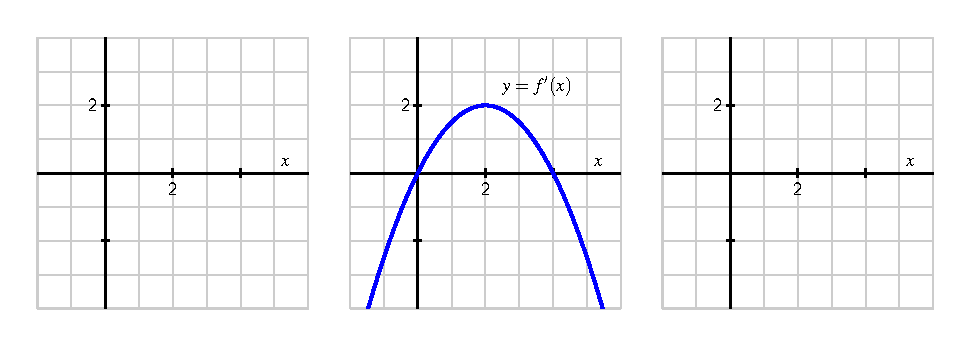
\includegraphics{figures/1_8_Act2.eps}}
\end{center}
\caption{At center, a graph of $y = f'(x)$; at left, axes for plotting $y = f(x)$; at right, axes for plotting $y = f''(x)$.} \label{F:1.8.Act2}
\end{figure}

Your task is to determine as much information as possible about $f$ (especially near the value $a = 2$) by responding to the questions below.
\ba
	\item Find a formula for the tangent line approximation, $L(x)$, to $f$ at the point $(2,-1)$.
	\item Use the tangent line approximation to estimate the value of $f(2.07)$.  Show your work carefully and clearly.
	\item Sketch a graph of $y = f''(x)$ on the righthand grid in Figure~\ref{F:1.8.Act2}; label it appropriately.
	\item Is the slope of the tangent line to $y = f(x)$ increasing, decreasing, or neither when $x = 2$?  Explain.
	\item Sketch a possible graph of $y = f(x)$ near $x = 2$ on the lefthand grid in Figure~\ref{F:1.8.Act2}.  Include a sketch of $y=L(x)$ (found in part (a)).  Explain how you know the graph of $y = f(x)$ looks like you have drawn it.   
	\item Does your estimate in (b) over- or under-estimate the true value of $f(2)$?  Why?
\ea
\end{activity}
\begin{smallhint}
\ba
	\item Find the value of $f'(2)$ from the given graph of $f$.
	\item Remember that $f(2.07) \approx L(2.07)$.
	\item The graph of $y = f''(x)$ is the derivative of the graph of $y = f'(x)$.
	\item Is $f'$ increasing, decreasing, or neither when $x = 2$? 
	\item Draw $y = L(x)$ first.  Then think about options for $f$ relative to the graph of $L$.  
	\item Does the tangent line lie above or below the graph of $y = f(x)$ at $(2,3)$?
\ea
\end{smallhint}
\begin{bighint}
\ba
	\item Find the value of $f'(2)$ from the given graph of $f$, and note that you are given that $f(2) = -1$.
	\item Remember that $f(2.07) \approx L(2.07)$.
	\item The graph of $y = f''(x)$ is the derivative of the graph of $y = f'(x)$.  Where must $f''(x) = 0$?  Where is $f''(x)$ positive?
	\item Is $f'$ increasing, decreasing, or neither when $x = 2$?  Use the given graph of $y = f'(x)$ to help you decide.
	\item Draw $y = L(x)$ first.  Then think about options for $f$ relative to the graph of $L$.  Is $f$ concave up or concave down before $x = 2$?  after $x = 2$?
	\item Does the tangent line lie above or below the graph of $y = f(x)$ at $(2,3)$?  You may have to consider values less than $x = 2$ and values greater than $x = 2$.
\ea
\end{bighint}
\begin{activitySolution}
\ba
	\item Since $f(2) = -1$ and $f'(2) = 2$, we have $L(x) = -1 + 2(x-2)$.
	\item Using our work in (a), $f(2.07) \approx L(2.07) = -1 + 2(2.07-2) = -1 + 2\cdot 0.07 = -0.86$.  
	\item See the plot below.
	\item Is the slope of the tangent line to $y = f(x)$ is increasing for $x < 2$ because $y = f'(x)$ is an increasing function on this interval.  Similarly, for $x > 2$, the slope of the tangent line to $y = f(x)$ is decreasing.  Right at $x = 2$, the slope of the tangent line to $y = f(x)$ is neither increasing nor decreasing.
	\item See the plot below.  Note that $y = f(x)$ is concave up for $x < 2$ since $f'$ is increasing on that interval, and $y = f(x)$ is concave down for $x > 2$ since $f'$ is decreasing there.  Hence $y = f(x)$ changes from concave up to concave down right at $x = 2$, which is also the point near 2 where the graph of $y = f(x)$ is steepest.
	\item Because the tangent line to $y = f(x)$ lies above the graph  of $f$ to the right of $x = 2$, our estimate of $f(2.07)$ is too large -- the local linearization overshoots the true value of $f$ at this point.
\ea

\begin{center}
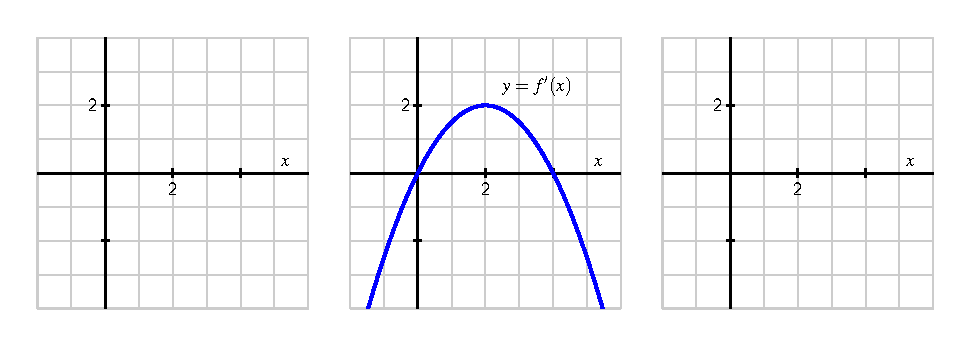
\includegraphics{figures/1_8_Act2.eps}
\end{center}
\end{activitySolution}
\aftera